\documentclass[12pt]{article}
\usepackage{blindtext}
\usepackage[en,bordered]{uni-style}
\usepackage{uni-math}
\usepackage{graphicx,wrapfig}


\title{Embedded Systems}
\prof{\href{https://scholar.google.com/citations?user=2RN0Y2YAAAAJ&hl=en}{\textcolor{black}{Prof. Sedighi}}}
\subtitle{Chapter 2 - Continuous Dynamics}
\subject{Homework 1}
\info{
    \begin{tabular}{lr}
        \href{https://github.com/M-Sc-AUT/M.Sc-Computer-Architecture/tree/main/Embedded Systems Modeling and Design}{\textcolor{black}{Reza Adinepour}} & ID: 402131055\\
    \end{tabular}
    }
    \date{\today}
    % \usepackage{xepersian}
    % \settextfont{Yas}
    \usepackage{uni-code}
    
    \begin{document}
\maketitlepage
\maketitlestart

\section{Question 2}

Show that if a system $S: A^\mathbb{R} \rightarrow B^\mathbb{R}$ is strictly causal and memoryless then its output is constant. Constant means that the output $(S(x))(t)$ at time $t$ does not depend on $t$.


\begin{qsolve}[Solution]
	
	\textbf{For Memoryless Systems I know:}
	
	a system has memory if the output depends not only on the current inputs, but
	also on past inputs (or future inputs, if the system is not causal). Consider we have a continuous time system like this: $ S: X \rightarrow Y $ where $ X=A^\mathbb{R} $ and $Y=B^\mathbb{R}$ for some sets $A$ and $B$. Formally, this system is \textbf{memoryless} if there exists a function $f: A \rightarrow B$ such that for all $x \in X$, 
	$$ (S(x)(t))=f(x(t)) $$
	
	for all $t \in \mathbb{R}$ That is, the output $(S(x))(t)$ at time t depends only on the input $x(t)$ at time $t$
	
	
	\textbf{and a system is causal if:}
	
	its output depends only on current and past inputs. it means:
	
	Consider a continuous-time system $ S: X \rightarrow Y $, where $X=A^\mathbb{R}$ and $Y=B^\mathbb{R}$ for same sets $A$ and $B$. This system is causal if for all $x1, x2 \in X$ and $\tau \in \mathbb{R}$
	
	$$ x_1|_{t < \tau} = x_2|_{t < \tau} \Rightarrow S(x_1)|_{t \le \tau} = S(x_2)|_{t \le \tau}$$
	
	--- Constant means that the output $(S(x))(t)$ at time $t$ does not depend on $t$.\\
	In this question we want a system that that has both of \textbf{memoryless} and \textbf{causality}.
	
	We need to show that for all $a_1, a_2 \in A, f(a_1)=f(a_2)$
	
	Using the function f , this becomes:
	$$ x_1|_{t < \tau} = x_2|_{t < \tau} \Rightarrow f(x_1)|_{t \le \tau} = f(x_2)|_{t \le \tau}$$
	
	for all $t\le \tau$. The left side of this expression imposes no constraint at all on the values of $x_1(\tau)$ and $x_2(\tau)$ so these can be arbitrary values $a_1, a_2 \in A$. Hence, the right hand side asserts that $f(a_1) = f (a_2)$ for all $a_1, a_2 \in A$.
	
	
\end{qsolve}
\vfil
%\begin{conclusion}
%	\blindtext
%\end{conclusion}
\clearpage







\section{Question 3}
This exercise studies linearity.

\begin{enumerate}
	\item Show that the helicopter model defined in Example 2.1 is linear if and only if
	the initial angular velocity $\dot{\theta}_{y}(0) = 0.$
	
	\begin{qsolve}[Solution]
		The helicopter model defined as bellow:
		$$\dot{\theta}_{y}(t) = \dot{\theta}_{y}(0) + \frac{1}{I_{yy}} \int_{0}^{t}T_y(\tau)d\tau$$
		
		for linear system we should prove this: (a and b is a constant)
		$$ ax_1(t)+bx_2(2) \rightarrow ay_1(t)+by_2(t) $$
		in this example we know:
		$$ x(t) = T_y(\tau) \\\ and \\\ y(t) = \dot{\theta}_{y}$$  
		
		in first i apply $ax_1(t)$ and $bx_2(t)$
		
		for $ax_1(t)$ we have:
		$$\dot{\theta}_{y1}(t) = \dot{\theta}_{y1}(0) + \frac{1}{I_{yy}} \int_{0}^{t}aT_{y1}(\tau)d\tau$$
		
		$$=\dot{\theta}_{y1}(t) = \dot{\theta}_{y1}(0) + \frac{a}{I_{yy}} \int_{0}^{t}T_{y1}(\tau)d\tau$$
		
		
		for $bx_2(t)$ we have:
		$$\dot{\theta}_{y2}(t) = \dot{\theta}_{y2}(0) + \frac{1}{I_{yy}} \int_{0}^{t}bT_{y2}(\tau)d\tau$$
		
		$$=\dot{\theta}_{y2}(t) = \dot{\theta}_{y2}(0) + \frac{b}{I_{yy}} \int_{0}^{t}T_{y2}(\tau)d\tau$$
		
		
		$$\rightarrow ax_1(t) + bx_2(t) = \dot{\theta}_{y1}(0) + \frac{a}{I_{yy}} \int_{0}^{t}T_{y1}(\tau)d\tau + \dot{\theta}_{y2}(0) + \frac{b}{I_{yy}} \int_{0}^{t}T_{y2}(\tau)d\tau$$
		
		$$ =\dot{\theta}_{y1}(0)+\dot{\theta}_{y2}(0)=\dot{\theta}_{y1}(0)+\dot{\theta}_{y2}(0)+\frac{1}{I_{y}}(a+b) \int_{0}^{t}T_{y1}(\tau)d\tau + \int_{0}^{t}T_{y2}(\tau)d\tau $$
		
		
		Now we should calculate $ay(t):$
		
		$$ a\dot{\theta}_{y1}(t) = a(\dot{\theta}_{y1}(t) = \dot{\theta}_{y1}(0) + \frac{1}{I_{yy}} \int_{0}^{t}T_{y1}(\tau)d\tau) = a\dot{\theta}_{y1}(0) + \frac{a}{I_{yy}}\int_{0}^{t}T_{y1}(\tau)d\tau $$
		
		
		$$ b\dot{\theta}_{y1}(t) = b(\dot{\theta}_{y1}(t) = \dot{\theta}_{y1}(0) + \frac{1}{I_{yy}} \int_{0}^{t}T_{y1}(\tau)d\tau) = b\dot{\theta}_{y1}(0) + \frac{b}{I_{yy}}\int_{0}^{t}T_{y1}(\tau)d\tau $$

	\end{qsolve}
	
	\begin{qsolve}[Solution]
		so:
		
		$$ a\dot{\theta}_{y1}(t)+b\dot{\theta}_{y1}(t) = a\dot{\theta}_{y1}(t)+b\dot{\theta}_{y2}(t)-\dot{\theta}_{y1}(0) \neq aT_{y1}(\tau)+bT_{y2}(\tau) $$
	\end{qsolve}
	
	
			
	
	\item Show that the cascade of any two linear actors is linear.
	
	
	\begin{qsolve}[Solution]
		As linearity defined before:
		
		$$ \forall x1, x2 \in X \\\ and \\\ \forall a, b \in \mathbb{R}: S(ax_1(t) + bx_2(t))=aS(x_1)+bS(x_2) $$
		
		then:
		
		$$ S_2(S_1(ax_1+bx_2)) = S_2(aS_1(s_1)+bS_1(x_2)) = aS_2(S_1(x_1))+bS_2(S_1(x_2))$$
	\end{qsolve}
	
	
	
	
	
	
	\item Augment the definition of linearity so that it applies to actors with two input
	signals and one output signal. Show that the adder actor is linear.
	
	\begin{qsolve}[Solution]
		A system model $S:X_1 \times X_2 \rightarrow Y$, where $X_1, X_2$, and $Y$ are sets of signals, is linear if it satisfies the superposition property:
		
		$$ \forall x_1, x'_1 \in X_1 \\\ and \\\ \forall  x_2, x'_2 \in X_2 \\\ and \\\ a,b \in \mathbb{R},$$
		
		$$ S(ax_1+bx'_1, ax_2+bx'_2)=aS(x_1,x_2)+bS(x'_1,x'_2) $$
		
		The adder component is given by:
		$$ S(x_1, x_2)=x_1+x_2 $$
		
		Hence:
		$$ S(ax_1+bx'_1, ax_2+bx'_2)=ax_1+bx'_1+ax_2+bx'_2=a(x_1+x_2)+b(x'_1+x'_2)$$
		$$ =aS(x_1,x_2)+bS(x'_1,x'_2) $$
		
	\end{qsolve}
\end{enumerate}



\vfil
\clearpage












\section{Question 4}
Consider the helicopter of Example 2.1, but with a slightly different definition of
the input and output. Suppose that, as in the example, the input is $T_y: \mathbb{R} \rightarrow \mathbb{R}$, as in the example, but the output is the position of the tail relative to the main rotor shaft. Specifically, let the $x-y$ plane be the plane orthogonal to the rotor shaft, and let the position of the tail at time $t$ be given by a tuple $((x(t), y(t)))$ Is this model LTI? Is it BIBO stable?



\begin{qsolve}[Solution]
	In this case, the system can be modeled as a function with two output signals as bellow:
	$$ S:(\mathbb{R} \rightarrow \mathbb{R}) \rightarrow (\mathbb{R} \rightarrow \mathbb{R})^2 $$
	where:
	$$ (S(T_y))(t)=(x(t), y(t)) $$
	where $(x(t), y(t))$ is the position of the tail in the $x-y$ plane. by changing the input torque, the output rotates in one plane, so the system \textbf{isn't linear}. I don't have any information about time invariancy of this system. but \textbf{this system is BIBO stable} because output of this system is bounded in the $x-y$ plane.
	
\end{qsolve}
\vfil
\clearpage

















\section{Question 5}
Consider a rotating robot where you can control the angular velocity around a fixed
axis.

\begin{enumerate}
	\item Model this as a system where the input is angular velocity $\dot{\theta}$ and the output is angle $\theta$ Give your model as an equation relating the input and output as functions of time.
	\begin{qsolve}[Solution]
		Input of this system is angular velocity $\dot{\theta}$ and the output is angle $\theta$. Since the output will be the integral of the input, we have:
		$$ \forall t \in \mathbb{R}, \theta(t)=\theta(0)+\int_{0}^{t}\dot{\theta(\tau)d\tau} $$
		where $\theta(0)$ is the initial position
		
	\end{qsolve}
	
	
	
	
	\item Is this model BIBO stable?
	\begin{qsolve}[Solution]
		As we know that integral with this limits is unstable system because the output tends to $\infty$, so it could be obviously seen that, this
		system \textbf{is not stable}.
		
		For example, the input:
		$$ \dot{\theta(t)=u(t)} $$
		
		is bounded but yields an unbounded output.
	\end{qsolve}
	
	
	
	
	
	\item Design a proportional controller to set the robot onto a desired angle. That is, assume that the initial angle is $\theta(0)=0$, and let the desired angle be $\psi(t)=au(t)$ where $u$ is the unit step function. Find the actual angle as a function of time and the proportional controller feedback gain $K$. What is your output at $t=0$? What does it approach as $t$ gets large?
	\begin{qsolve}[Solution]
		We can design proportional controller as bellow:\\
		
		
		
		
		\centering\includegraphics*[width=0.6\linewidth]{images/img2}
		\captionof{figure}{Proportional controller}
		

		
		\raggedright According to example 2.6 in page 33, we can write:
		$$ \theta(t)=k_p\int_{0}^{t}(\psi(\tau)-\theta(\tau))d\tau=k_p\int_{0}^{t}(au(t)-\theta(\tau))d\tau $$
		$$ \theta(t)=au(t)(1-e^{-k_pt}) $$
		
		The output at $\theta(0^-)=\theta(0^+)=0$, as expected. As $t$ gets large, the output approaches $a$.
		
	\end{qsolve}
\end{enumerate}




\vfil
\clearpage


















\section{Question 6}
A DC motor produces a torque that is proportional to the current through the windings of the motor. Neglecting friction, the net torque on the motor, therefore, is this torque minus the torque applied by whatever load is connected to the motor. Newton’s second law (the rotational version) gives

$$ k_{T}i(t)-x(t)=I\frac{d}{dt}\omega(t) $$

where $k_T$ is the motor torque constant, $i(t)$ is the current at time $t$, $x(t)$ is the torque
applied by the load at time $t$, $I$ is the moment of inertia of the motor, and $\omega(t)$ is
the angular velocity of the motor.



\begin{enumerate}
	\item Assuming the motor is initially at rest, rewrite (2.15) as an integral equation.
	\begin{qsolve}[Solution]
		Assuming the motor is initially at rest, rewrite (2.15) as an integral equation.
		$$ \int_{0}^{t}(K_Ti(t)-x(t))dt=\int_{0}^{t}(I\frac{d}{dt}\omega(t))dt $$
		$$ \int_{0}^{t}(K_Ti(t)-x(t))dt=I\omega(t) \Rightarrow \omega(t)=\frac{1}{I}\int_{0}^{t}(K_Ti(t)-x(t))dt $$
	\end{qsolve}
	
	
	
	
	
	
	
	\item Assuming that both $x$ and $i$ are inputs and $\omega$ is an output, construct an actor
	model (a block diagram) that models this motor. You should use only prim-
	itive actors such as integrators and basic arithmetic actors such as scale and
	adder.
	\begin{qsolve}[Solution]
		
		\centering\includegraphics*[width=1\linewidth]{images/img3}
		\captionof{figure}{Block diagram of model}
	\end{qsolve}
	
	
	
	\item In reality, the input to a DC motor is not a current, but is rather a voltage. If
	we assume that the inductance of the motor windings is negligible, then the
	relationship between voltage and current is given by
\end{enumerate}

$$ v(t)=R_i(t)+k_b\omega(t) $$

where $R$ is the resistance of the motor windings and $k_b$ is a constant called the
motor back electromagnetic force constant. The second term appears because
a rotating motor also functions as an electrical generator, where the voltage
generated is proportional to the angular velocity.

Modify your actor model so that the inputs are $v$ and $x$ rather than $i$ and $x$.



\begin{qsolve}[Solution]
	
	\centering\includegraphics*[width=1\linewidth]{images/img4}
	\captionof{figure}{Block diagram of model}
\end{qsolve}
\vfil
\clearpage






















\section{Question 7}


\begin{enumerate}
	\item Using your favorite continuous-time modeling software (such as LabVIEW,
	Simulink, or Ptolemy II), construct a model of the helicopter control system
	shown in Figure 2.4. Choose some reasonable parameters and plot the actual
	angular velocity as a function of time, assuming that the desired angular veloc-
	ity is zero, $\psi(t)=0$, and that the top-rotor torque is non-zero, $T_t(t) = bu(t)$.
	Give your plot for several values of $K$ and discuss how the behavior varies
	with $K$.
	
	\item Modify the model of part 1 to replace the Controller of Figure 2.4 (the sim-
	ple scale-by-$K$ actor) with the alternative controller shown in Figure 2.6. This alternative controller is called a \textbf{proportional-integrator (PI) controller}. It
	has two parameter $K1$ and $K2$ . Experiment with the values of these parame-
	ters, give some plots of the behavior with the same inputs as in part 1, and
	discuss the behavior of this controller in contrast to the one of part 1.
\end{enumerate}

\begin{figure}[h]
	\centering
	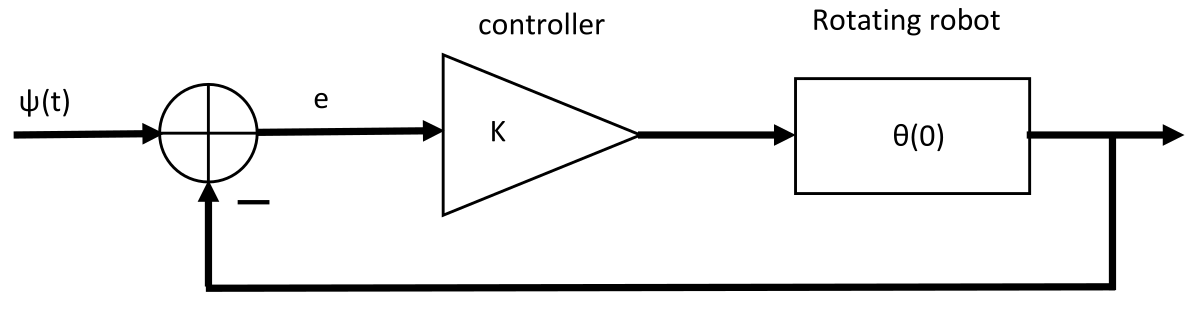
\includegraphics[width=0.7\textwidth]{images/img2}
	\caption{A PI controller for the helicopter}
	\label{fig:A PI controller for the helicopter}
\end{figure}



\begin{qsolve}[Solution]
	For this question i use MATLAB SIMULINK. Design model of helicopter controller as bellow:\\
	
	\centering\includegraphics*[width=1\linewidth]{images/img5}
	\captionof{figure}{Simulink model of PI controller}
	
	
	\raggedright the output of the system is shown below:
	
	\centering\includegraphics*[width=1\linewidth]{images/Q7_result}
	\captionof{figure}{Output of controller}
	
	
	\raggedright With the controller gains set to $K_1 = K_2 = 10$ and the top rotor torque at $T_t(t)=0.5u(t)$, we see that the angular velocity settles eventually to zero. Increasing $K_1$ results in a smaller peak error. Increasing $K_2$ results in fast settling, but also some overshoot.
	
	
\end{qsolve}
\vfil
\clearpage




\vspace*{\fill}
\begin{center}
	\makeendpage

\end{center}
\vfill % equivalent to \vspace{\fill}
\clearpage




\end{document}